\documentclass[10pt,a4paper,twocolumn]{article}
\usepackage[T1]{fontenc}
\usepackage[utf8]{inputenc}
\usepackage{lmodern}
\usepackage[margin=0.75in,columnsep=0.3in]{geometry}
\usepackage{dblfloatfix}
\usepackage{amsmath,amssymb}
\usepackage{graphicx}
\usepackage{booktabs}
\usepackage{tabularx}
\usepackage{array}
\usepackage[round]{natbib}
\usepackage[hidelinks]{hyperref}
\usepackage{microtype}
\usepackage{xcolor}
\usepackage{tikz}
\usetikzlibrary{positioning,arrows.meta,fit,calc}

\setlength{\parskip}{0.2em}
\raggedbottom
\newcolumntype{Y}{>{\raggedright\arraybackslash}X}

\newcommand{\Eq}{\textsc{Eq}}
\newcommand{\Fwd}{\textsc{Fwd}}
\newcommand{\Bwd}{\textsc{Bwd}}
\newcommand{\Neg}{\textsc{Neg}}
\newcommand{\sd}[1]{\,{\scriptsize$\pm$#1}}

\title{Stronger Encoders and Structure-Constrained Decoding\\ for DiCo-NLI (Track 1)}
\author{Muhammad Muneeb Baig, Syed Kamran Ali Shah, Kashaf Ali Haroon\\ MS Data Science, SEECS, NUST\\ CS-878 Deep Learning, Assignment 2: Proposed Approach and Experimental Design}
\date{November 2026}

\begin{document}
\maketitle

\begin{abstract}
Assignment~1 (A1) established that a fine-tuned RoBERTa-base reaches 0.765 weighted F1 (W-F1) and 0.739 HardCons on the DiCo-NLI English development set, and that its remaining errors lie mostly on the \Neg{} boundary rather than on direction. We propose a pair-aware system: a fully fine-tuned DeBERTa-v3 cross-encoder that sees both orientations of a pair in the same batch, an optional reversal-consistency loss, \Neg{} class weighting, and inference-time decoding rules that decide both orientations together. We define comparison systems, an ablation plan, the evaluation measures and a complete protocol, and verify an end-to-end implementation. In preliminary three-seed runs, DeBERTa-v3 improves argmax W-F1 from 0.758 to 0.821 and HardCons from 0.759 to 0.839 (both significant under a paired bootstrap). Symmetric decoding adds 2.3 HardCons points at no training cost. A property of the released data (rows with a reversed partner are never \Neg) gives the largest gain, to 0.925 W-F1, but it is dataset-specific. The consistency loss shows no significant effect. These are verification results on a development set that informed our design, not final performance claims.
\end{abstract}

\section{Proposed Approach}
\label{sec:approach}

\textbf{Task.} The input is an ordered pair of short English phrases $(t_1,t_2)$; the output is one of four labels for that ordered pair: \Eq{} (equivalence), \Fwd{} ($t_1$ entails $t_2$), \Bwd{} ($t_2$ entails $t_1$) or \Neg{} (opposition, similarity, relatedness or no relation, merged into one class) \citep{diconli2026,maccartney2009natural}. The prediction target is one label per row. Many pairs appear in both orientations, and a correct system must then satisfy the reversal rule $f(t_2,t_1)=\mathrm{rev}(f(t_1,t_2))$, with $\mathrm{rev}(\Fwd)=\Bwd$, $\mathrm{rev}(\Bwd)=\Fwd$ and $\mathrm{rev}(\Eq)=\Eq$. The expected model behaviour is therefore not only a correct label per row but coherent labels across orientations.

\textbf{System overview.} The system has four parts (Figure~\ref{fig:arch}): (1) \emph{pair-aware preprocessing}, which groups the two orientations of a pair by \texttt{pair\_id} and tokenizes each orientation as one cross-encoder input; (2) a \emph{fully fine-tuned DeBERTa-v3-base} encoder with a classification head; (3) a \emph{training objective} of class-weighted cross-entropy plus an optional reversal-consistency term; and (4) a \emph{pair-aware decoder} that chooses labels for both orientations together.

\textbf{Role of the A1 features.} A1's most informative engineered features were directional: phrase lengths, word coverage of one phrase by the other, and containment. A cross-encoder reads both phrases jointly with cross-attention, so it can learn these signals from the tokens; we do not feed them explicitly. They remain in the classical comparison system (Section~\ref{sec:comparison}), which makes it possible to see what the encoder adds beyond them.

\textbf{Preprocessing, augmentation and sampling.} There is no text normalization: the tokenizers are cased and the phrases are used as released. Each row becomes ``[CLS] $t_1$ [SEP] $t_2$ [SEP]'', truncated at 64 tokens. The longest dev pair has 18 words (mean 5.9), so the limit is not expected to bind. We do not use reversal augmentation: 1,282 of the 1,760 training pairs already appear in both orientations, so reversing them would only duplicate data. Reversing the 478 single \Neg{} rows would also create \Neg{} rows with partners, which never occur in the released data. Instead, batches are sampled by pair: a reversible pair always contributes both orientations to the same batch, and batches are shuffled each epoch. There is no feature selection.

\textbf{Variation and noise.} \emph{Imbalance:} \Neg{} is the smallest class (16\% of train) and the hardest; we weight it in the loss and report Macro-F1 alongside W-F1. \emph{Noisy labels:} some gold labels are debatable (A1 found near-paraphrases labelled \Neg); we do not model label noise, but an audit is planned (Section~\ref{sec:plan}). \emph{Long inputs:} not an issue at 18 words. \emph{Cross-lingual variation:} this system covers Track~1 only; a multilingual pilot is planned. Domain, speaker and multimodal variation do not apply to this task.

\textbf{Expected limitations and sources of error.} (i) The \Eq/\Fwd/\Bwd{} boundary for near-paraphrases, where a small word difference may or may not change entailment; (ii) the heterogeneous \Neg{} class, which merges four relations; (iii) dependence of the structural decoding rules on how the dataset was built; (iv) the small training set (2,738 rows after the validation split).

\section{Method Justification}
\label{sec:just}

Table~\ref{tab:just} links each design decision to evidence from A1. We follow the pattern observation $\rightarrow$ interpretation $\rightarrow$ modelling implication.

\begin{table*}[!t]
\centering
\small
\begin{tabularx}{\textwidth}{>{\raggedright\arraybackslash}p{4.6cm} >{\raggedright\arraybackslash}p{4.4cm} Y}
\toprule
Evidence from A1 or the data & Design decision & Expected effect \\\addlinespace[3pt]
\midrule\addlinespace[1pt]
\Neg{} is the weakest class (RoBERTa F1 0.565) and the smallest (16\% of train) & \Neg{} class weight $w_{\Neg}=2$ in the loss; report Macro-F1 and per-class recall & Higher \Neg{} recall; less dominance of the three larger classes \\\addlinespace[3pt]
69 near-paraphrases rejected as \Neg; \Eq{} F1 only 0.725 & Stronger encoder: DeBERTa-v3-base \citep{he2023debertav3} & Better separation of \Eq{} from \Neg{} on lexically similar pairs \\\addlinespace[3pt]
\Fwd/\Bwd{} confused only twice in each direction, but 15--19 pairs per seed are \Neg{} in exactly one orientation & Decide both orientations jointly: pair-aware batching, consistency loss, symmetric decoding & Remove one-sided errors; raise HardCons without hurting W-F1 \\\addlinespace[3pt]
Length-only LR: SoftCons 0.989 but W-F1 0.464 & Judge every change on W-F1 and HardCons together, never SoftCons alone & Avoid rewarding systems that are consistent but wrong \\\addlinespace[3pt]
In train and dev, every row with a reversed partner is non-\Neg{} and every row without one is \Neg & Structure-constrained decoding, reported separately from model gains & Large \Neg{} gain on dev; transfers to test only if the test file is built the same way \\\addlinespace[3pt]
Train already holds both orientations of 1,282 pairs & No reversal augmentation; sample whole pairs instead & Consistency loss computable without extra data \\\addlinespace[3pt]
DeBERTa-v3 gave NaN losses on Apple MPS in A1 & Train in fp32 on CUDA, with gradient clipping & Stable DeBERTa training \\\addlinespace[3pt]
\bottomrule
\end{tabularx}
\caption{Evidence from A1, the design decision it motivates, and the expected effect.}
\label{tab:just}
\end{table*}

\textbf{Encoder.} \emph{Observation:} A1's errors concentrate on \Eq{} versus \Neg{} for lexically similar phrases. \emph{Interpretation:} the model must judge whether a small lexical change alters meaning, which depends on word order and relative position. \emph{Implication:} DeBERTa-v3 encodes content and relative position separately (disentangled attention) and is pretrained with replaced-token detection \citep{he2023debertav3}. It was also the strongest model in the organisers' pilot \citep{apaolaza2026assessing}. We test whether that translates into a better \Eq/\Neg{} boundary, rather than assuming it.

\textbf{Joint decisions over both orientations.} \emph{Observation:} RoBERTa almost never swaps \Fwd{} and \Bwd, yet still loses SoftCons and HardCons on pairs where one orientation is called \Neg. \emph{Interpretation:} the two orientations are scored independently, so nothing forces their decisions to agree. \emph{Implication:} make the decision at pair level, during training (a consistency regulariser, in the spirit of logic-constrained NLI training \citep{minervini2018adversarially,li2019logic}) and at inference (symmetric decoding). Consistency benchmarks show that pretrained models are often inconsistent under such transformations \citep{jang2022becel}.

\textbf{Pair structure.} \emph{Observation:} the training set has 1,282 pairs in both orientations ($2\times1{,}282=2{,}564$ rows) and 478 rows in one orientation only; all 478 are \Neg, and no paired row is \Neg. Dev shows the same pattern (277 pairs, 106 single \Neg{} rows). \emph{Interpretation:} this is a construction artifact of the dataset, similar to the annotation artifacts found in other NLI datasets \citep{gururangan2018annotation}. Partners can be found from \texttt{pair\_id} in the participant file, which is available at test time, without any gold label. \emph{Implication:} decoding rules that use it can be applied, but they must be reported separately and described as dataset-specific. It also explains why most top development-leaderboard entries (9 of the other 25 English submissions on 8 November) report SoftCons of exactly 1.0: SoftCons fails a pair whenever either prediction is \Neg.

\section{System Architecture}
\label{sec:arch}

\begin{figure*}[!t]
\centering
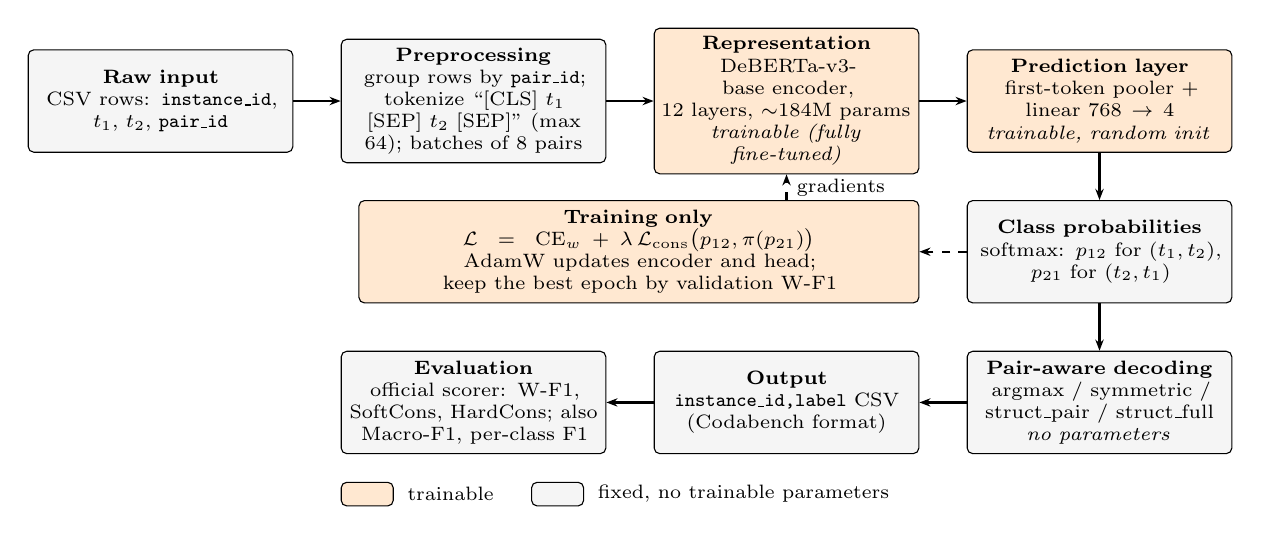
\begin{tikzpicture}[
  box/.style={draw,rounded corners=2pt,align=center,font=\scriptsize,text width=3.15cm,minimum height=1.3cm,inner sep=3pt},
  tr/.style={box,fill=orange!18},
  fx/.style={box,fill=gray!8},
  arr/.style={-{Stealth[length=4pt]},thick},
  node distance=0.6cm]
% row 1: input to prediction layer
\node[fx] (raw) {\textbf{Raw input}\\ CSV rows: \texttt{instance\_id},\\ $t_1$, $t_2$, \texttt{pair\_id}};
\node[fx,right=of raw] (pre) {\textbf{Preprocessing}\\ group rows by \texttt{pair\_id}; tokenize ``[CLS] $t_1$ [SEP] $t_2$ [SEP]'' (max 64); batches of 8 pairs};
\node[tr,right=of pre] (enc) {\textbf{Representation}\\ DeBERTa-v3-base encoder,\\ 12 layers, $\sim$184M params\\ \emph{trainable (fully fine-tuned)}};
\node[tr,right=of enc] (head) {\textbf{Prediction layer}\\ first-token pooler +\\ linear $768\!\to\!4$\\ \emph{trainable, random init}};
% row 2: probabilities and training branch
\node[fx,below=0.6cm of head] (sm) {\textbf{Class probabilities}\\ softmax: $p_{12}$ for $(t_1,t_2)$,\\ $p_{21}$ for $(t_2,t_1)$};
\node[tr,left=of sm,text width=6.9cm,minimum height=1.3cm] (loss) {\textbf{Training only}\\ $\mathcal{L}=\mathrm{CE}_w+\lambda\,\mathcal{L}_{\mathrm{cons}}\big(p_{12},\pi(p_{21})\big)$\\ AdamW updates encoder and head; keep the best epoch by validation W-F1};
% row 3: decoding to evaluation
\node[fx,below=0.6cm of sm] (dec) {\textbf{Pair-aware decoding}\\ argmax / symmetric /\\ struct\_pair / struct\_full\\ \emph{no parameters}};
\node[fx,left=of dec] (out) {\textbf{Output}\\ \texttt{instance\_id,label} CSV\\ (Codabench format)};
\node[fx,left=of out] (ev) {\textbf{Evaluation}\\ official scorer: W-F1, SoftCons, HardCons; also Macro-F1, per-class F1};
\draw[arr] (raw) -- (pre); \draw[arr] (pre) -- (enc); \draw[arr] (enc) -- (head);
\draw[arr] (head) -- (sm); \draw[arr] (sm) -- (dec); \draw[arr] (dec) -- (out); \draw[arr] (out) -- (ev);
\draw[arr,dashed] (sm) -- (loss);
\draw[arr,dashed] (loss.north -| enc) -- node[right,font=\scriptsize]{gradients} (enc.south);
% legend
\node[tr,minimum height=0.3cm,text width=0.45cm,below=0.35cm of ev.south west,anchor=north west] (lg1) {};
\node[right=0.05cm of lg1,font=\scriptsize] (lg1t) {trainable};
\node[fx,minimum height=0.3cm,text width=0.45cm,right=0.35cm of lg1t] (lg2) {};
\node[right=0.05cm of lg2,font=\scriptsize] {fixed, no trainable parameters};
\end{tikzpicture}
\caption{Proposed system. Both orientations of a pair pass through the same encoder and head in the same batch. Nothing is frozen: all encoder and head parameters are updated. $\pi$ swaps the \Fwd{} and \Bwd{} probabilities. Single (\Neg) rows receive only the cross-entropy term. The decoding rules and the scorer have no trainable parameters.}
\label{fig:arch}
\end{figure*}

\textbf{Encoder and head.} We use \texttt{AutoModelForSequenceClassification} with the pretrained \texttt{microsoft/deberta-v3-base} weights (about 184M parameters, of which about 98M are the 128k-token embedding matrix). The head takes the first-token representation, applies a dense layer with GELU (the DeBERTa pooler) and a linear layer to four logits. The head is initialised randomly; dropout is the model default (0.1). For RoBERTa the structure is the same, with its own classification head.

\textbf{Training objective.} Let $p_{12}=\mathrm{softmax}(f_\theta(t_1,t_2))$ and $p_{21}=\mathrm{softmax}(f_\theta(t_2,t_1))$. Let $\pi$ be the label permutation that maps a distribution for $(t_2,t_1)$ onto the label space of $(t_1,t_2)$: it keeps \Eq{} and \Neg{} and swaps \Fwd{} and \Bwd. For each reversible pair in a batch,
\begin{equation}
\mathcal{L}_{\mathrm{cons}}=\tfrac12\Big[\mathrm{KL}\big(p_{12}\,\|\,\pi(p_{21})\big)+\mathrm{KL}\big(\pi(p_{21})\,\|\,p_{12}\big)\Big],
\end{equation}
and the loss for a batch is
\begin{equation}
\mathcal{L}=\mathrm{CE}_w(y,p)+\lambda\,\overline{\mathcal{L}_{\mathrm{cons}}},
\end{equation}
where $\mathrm{CE}_w$ is cross-entropy over all rows, with weight $w_{\Neg}$ on \Neg{} and 1 elsewhere, and the bar denotes the mean over reversible pairs in the batch. Single rows have no partner, so they receive only $\mathrm{CE}_w$.

\textbf{Decoding rules.} These change only how labels are chosen, so they apply to any trained model:
\begin{itemize}\setlength\itemsep{0pt}
\item \textbf{argmax}: $\hat y=\arg\max p_{12}$, as in A1.
\item \textbf{symmetric}: for a row with a partner, $\tilde p_{12}=\tfrac12\big(p_{12}+\pi(p_{21})\big)$ and the partner receives $\pi(\tilde p_{12})$, so the two labels are consistent by construction.
\item \textbf{struct\_pair}: symmetric, and rows with a partner may not be \Neg.
\item \textbf{struct\_full}: struct\_pair, and rows without a partner are labelled \Neg.
\end{itemize}
The last two use the pair structure of Section~\ref{sec:just}. struct\_full changes only rows without a partner, which never enter SoftCons or HardCons, so it can raise W-F1 but not HardCons relative to struct\_pair.

\section{Comparison Systems}
\label{sec:comparison}

All systems are scored on the same official dev set with the same scorer (Table~\ref{tab:systems}).

\textbf{Simple baselines.} The \emph{majority class} predicts \Fwd{} for every row. Its accuracy (0.288) equals the \Fwd{} share of dev, and its W-F1 (0.129) shows that no single label dominates: \Fwd, \Bwd{} and \Eq{} each cover 26--29\% of dev, and \Neg{} 16\%. A \emph{length-only} logistic regression tests the heuristic ``the longer phrase entails the shorter''. It is highly consistent (SoftCons 0.989) but mostly wrong (W-F1 0.464), which is why SoftCons alone cannot be used to compare systems.

\textbf{Classical baselines.} Logistic regression (L2, $C=1$, L-BFGS, 5,000 iterations, no class weighting) on (a) 16 standardised engineered features (phrase lengths and differences, word coverage and containment in both directions, extra words on each side, Jaccard overlap, identity, negation and number mismatch), (b) TF-IDF unigrams and bigrams with sublinear term frequency, using separate blocks for $t_1$ and $t_2$ so that direction is preserved, and (c) both together. These were trained on the full training set in A1.

\textbf{Pretrained baselines.} BERT-base-uncased and RoBERTa-base, fully fine-tuned as cross-encoders with a linear head on the first token and cross-entropy (A1 protocol: AdamW, learning rate $3\times10^{-5}$, batch 16, 6 epochs, final epoch kept by a rule fixed in advance, Apple M4 GPU). \textbf{M0} retrains RoBERTa-base under the A2 protocol, so that the proposed systems can be compared with it on identical splits.

\textbf{Proposed systems.} \textbf{M1}: DeBERTa-v3-base, cross-entropy only. \textbf{M2}: M1 + consistency loss ($\lambda=1$). \textbf{M2b}: $\lambda=0.5$, one seed, as a sensitivity check. \textbf{M3}: M2 + \Neg{} weighting ($w_{\Neg}=2$). Each is evaluated under all four decoding rules, and as a three-seed probability ensemble. What distinguishes them from the baselines is the pair-level treatment of the task, in training (pair-aware batching and the consistency loss) and at inference (pair-aware decoding).

\begin{table}[!t]
\centering
\small
\setlength{\tabcolsep}{3.5pt}
\begin{tabular}{l ccc}
\toprule
System (argmax) & W-F1 & Soft & Hard \\
\midrule
Majority class & 0.129 & 0.000 & 0.000 \\
LR, length only & 0.464 & 0.989 & 0.628 \\
LR, engineered features & 0.593 & 0.877 & 0.653 \\
LR, TF-IDF + features & 0.620 & 0.856 & 0.661 \\
BERT-base (A1) & 0.705 & 0.774 & 0.693 \\
RoBERTa-base (A1) & 0.765 & 0.804 & 0.739 \\
\midrule
M0 RoBERTa, A2 protocol & 0.758 & 0.819 & 0.759 \\
M1 DeBERTa-v3 & 0.821 & 0.892 & 0.839 \\
M3 + cons. + \Neg{} wt. & 0.827 & 0.878 & 0.828 \\
\bottomrule
\end{tabular}
\caption{Comparison systems on dev (official scorer). Soft/Hard: SoftCons/HardCons. A1 rows are from A1; neural rows are three-seed means. Results under the other decoding rules are in Table~\ref{tab:main}.}
\label{tab:systems}
\end{table}

\section{Ablation Plan}
\label{sec:ablation}

Each ablation changes one component and answers one question (Table~\ref{tab:ablation}). Ablations A--F are run in this assignment as preliminary checks; G--L are planned for A3.

\begin{table*}[!t]
\centering
\small
\begin{tabularx}{\textwidth}{c >{\raggedright\arraybackslash}p{3.7cm} >{\raggedright\arraybackslash}p{4.6cm} Y}
\toprule
ID & Ablation & Hypothesis & Expected interpretation / preliminary outcome \\
\midrule
A & RoBERTa (M0) vs DeBERTa-v3 (M1) & A stronger encoder improves the \Eq/\Neg{} boundary & Gain isolates the encoder. \emph{Done:} +6.3 W-F1, +7.9 HardCons, both significant \\
B & Consistency loss on/off (M1 vs M2) & Training-time agreement raises HardCons & Gain isolates the loss. \emph{Done:} no significant effect \\
C & $\lambda=1$ vs $\lambda=0.5$ & The loss is not over- or under-weighted & Sensitivity of B to its weight. \emph{Done, one seed:} no improvement \\
D & \Neg{} weighting on/off (M2 vs M3) & Weighting raises \Neg{} recall without hurting other classes & Inspect \Neg{} precision/recall. \emph{Done:} recall up, W-F1 change not significant \\
E & Decoding rule: argmax / symmetric / struct\_pair / struct\_full & Joint decisions remove one-sided errors; structure decides \Neg & Separates model gains from inference gains. \emph{Done:} both significant \\
F & Single seed vs three-seed ensemble & Averaging reduces seed variance & \emph{Done:} +1.1 W-F1, significant \\
\midrule
G & Frozen encoder (linear probe) vs fully fine-tuned & Task adaptation is needed beyond generic representations & Accuracy gain against training cost \\
H & Generic vs NLI-pretrained initialisation (MNLI-style checkpoint) & Prior entailment training helps the \Eq/\Fwd/\Bwd{} decision & Gain on paired rows \\
I & Four-class vs three-class model on paired rows only & When \Neg{} is decided structurally, the model need not learn it & Gain on \Eq/\Fwd/\Bwd; removes ``\Neg{} both ways'' \\
J & Checkpoint selection under argmax vs under the final decoding rule & Selection should match the deployed rule & Different epochs selected; effect on dev \\
K & Averaged vs joint pair decoding (best of 3 valid labelings) & Exact pair-level decoding beats averaging & Change in HardCons \\
L & Base vs large encoder; same- vs cross-backbone ensembles & Capacity and diversity help & Gain against cost \\
\bottomrule
\end{tabularx}
\caption{Ablation plan. Significance is judged with the paired cluster bootstrap of Section~\ref{sec:eval}; preliminary outcomes are detailed in Section~\ref{sec:results}.}
\label{tab:ablation}
\end{table*}

\section{Evaluation Measures}
\label{sec:eval}

\subsection{Official metrics}

All three official metrics are higher-is-better and range from 0 to 1. For class $c$ with precision $P_c$, recall $R_c$ and gold support $n_c$ among $N$ rows,
\begin{equation}
\mathrm{F1}_c=\frac{2P_cR_c}{P_c+R_c},\qquad \text{W-F1}=\sum_{c}\frac{n_c}{N}\,\mathrm{F1}_c .
\end{equation}
\textbf{W-F1} is the main score. Because it weights classes by support, the three large classes (84\% of dev) dominate it, and a weak minority class costs relatively little; we therefore also report Macro-F1.

Let $\mathcal{R}$ be the set of reversible dev pairs ($|\mathcal{R}|=277$), with gold labels $(y_{12},y_{21})$ and predictions $(\hat y_{12},\hat y_{21})$. Then
\begin{align}
\text{SoftCons}&=\frac{1}{|\mathcal{R}|}\sum_{\mathcal{R}}\mathbf{1}\big[\hat y_{12}\neq\Neg\ \wedge\ \hat y_{21}=\mathrm{rev}(\hat y_{12})\big],\\
\text{HardCons}&=\frac{1}{|\mathcal{R}|}\sum_{\mathcal{R}}\mathbf{1}\big[\hat y_{12}=y_{12}\ \wedge\ \hat y_{21}=y_{21}\big].
\end{align}
\textbf{SoftCons} rewards coherent predictions and ignores gold labels, so it can be high for a wrong system. \textbf{HardCons} rewards pairs that are both coherent and correct, so $\text{HardCons}\le\text{SoftCons}$ when gold is coherent. Both are computed only over reversible pairs, which in dev are all non-\Neg; single rows affect only W-F1. All three are averaged over items, not over classes.

\subsection{Secondary metrics}

Accuracy; Macro-F1, which weights the four classes equally and is therefore sensitive to \Neg; per-class precision, recall and F1; and the number of strictly one-sided \Neg{} pairs (one orientation \Neg, the other not), which isolates the error type that motivated the method.

\textbf{Uncertainty.} We report mean $\pm$ sample standard deviation over three seeds. For comparisons we use a paired cluster bootstrap: we resample the 383 dev \texttt{pair\_id} groups (277 pairs and 106 single rows) with replacement 2,000 times, keeping both orientations of a pair together, and recompute the seed-averaged difference between two systems on each resample. We report the 95\% percentile interval and a one-sided bootstrap $p$ value. This measures uncertainty from the finite dev set; seed variance is reported separately.

\subsection{Subgroup and robustness analysis}

We report accuracy by label, by pair type (rows with and without a partner), by pair length (total words, in thirds) and by lexical overlap (word Jaccard, in thirds). These groups test whether the aggregate score hides weak spots: pairs without a partner are all \Neg, long pairs contain more content to compare, and low-overlap pairs cannot be solved by word matching.

\section{Experimental Protocol}
\label{sec:protocol}

\begin{table}[!t]
\centering
\small
\begin{tabularx}{\columnwidth}{>{\raggedright\arraybackslash}p{2.35cm} Y}
\toprule
Setting & Value \\
\midrule
Data & DiCo-NLI Track 1 (English), organisers' release (GitHub, commit \texttt{588968e}, 8 Sep 2026) \\
Partitions & train 3,042 rows; dev 660 (277 pairs + 106 singles); test hidden until Jan 2027 \\
Validation & 10\% of train by \texttt{pair\_id}: 128 pairs + 48 singles (304 rows); split seed 2027, identical for all runs \\
Tokenization & model tokenizer, cased; pair input; max 64 tokens; dynamic padding \\
Initialisation & pretrained Hub checkpoints; head random \\
Optimiser & AdamW, lr $2\times10^{-5}$, weight decay 0.01 \\
Schedule & linear warm-up (10\% of steps), linear decay \\
Batch & 8 pairs ($\approx$16 rows), shuffled per epoch \\
Regularisation & dropout 0.1 (default); grad.\ clip 1.0 \\
Epochs / selection & 6 epochs; keep the epoch with the best validation argmax W-F1 \\
Loss settings & $\lambda\in\{0,0.5,1\}$, $w_{\Neg}\in\{1,2\}$ \\
Precision & fp32 \\
Seeds & 13, 42, 87 \\
Hardware & Google Colab, NVIDIA T4 (16\,GB) \\
Software & Python 3, PyTorch and Hugging Face Transformers (Colab defaults, Nov.\ 2026), scikit-learn \\
Cost & $\approx$2 min per RoBERTa run, 3.3 min per DeBERTa run (6 epochs) \\
\bottomrule
\end{tabularx}
\caption{Training and evaluation configuration, shared by all A2 runs.}
\label{tab:config}
\end{table}

Table~\ref{tab:config} lists the configuration used for every A2 run.

\textbf{Hyperparameter search.} None. The optimiser settings follow A1 and common fine-tuning defaults, and $\lambda$ and $w_{\Neg}$ were fixed before training; the only variation is the single-seed $\lambda=0.5$ check. This avoids tuning on dev, and leaves a search on the validation split for A3.

\textbf{Model selection.} After each epoch we compute argmax W-F1 on the validation split and keep the best epoch. Dev is never used to select checkpoints or set hyperparameters.

\textbf{Missing and duplicated instances.} No row or label is missing. Seven dev rows repeat a training pair exactly (15 if case is ignored, from 8 \texttt{pair\_id}s), always with the same label. We keep them, because the official evaluation includes them; they make up 2.3\% of dev and slightly favour any trained model.

\textbf{Class imbalance.} \Neg{} weighting in M3, and Macro-F1 and per-class recall in reporting. No resampling.

\textbf{Leakage prevention.} (i) The validation split is grouped by \texttt{pair\_id}, so a pair and its reverse are never split across training and validation. (ii) Train and dev share no \texttt{pair\_id}. (iii) The decoding rules find partners only from \texttt{pair\_id} in the participant file, never from gold labels. (iv) Checkpoints and settings are never chosen on dev. (v) The test set has not been seen.

\textbf{Local versus server evaluation.} Local evaluation runs the organisers' scorer on the public dev labels. We verified that it reproduces the Codabench development-phase score exactly. Hidden-test scores will come only from the server during the official evaluation window (January 2027).

\textbf{Use of dev.} Although dev was not used for selection, it was used to compare decoding rules and configurations, so the final configuration is informed by dev results. Dev scores are therefore not an independent estimate of test performance.

\section{Initial Implementation}
\label{sec:impl}

The system runs end to end in PyTorch and Hugging Face Transformers (Table~\ref{tab:impl}). One Colab notebook drives all experiments and the submission file.

\begin{table}[!t]
\centering
\small
\begin{tabularx}{\columnwidth}{>{\raggedright\arraybackslash}p{2.3cm} Y}
\toprule
Requirement & Implementation \\
\midrule
Data loading & \texttt{src/data.py}: official CSVs, label map \\
Preprocessing, representation & \texttt{PairCollator}: pairs by \texttt{pair\_id}, tokenizes both orientations \\
Model, training & \texttt{src/train\_a2.py}: \texttt{run(**config)}, loss, validation selection \\
Inference & \texttt{predict\_probs}; probabilities saved per run \\
Decoding & \texttt{src/decoding.py}: four rules \\
Evaluation & official scorer; \texttt{06\_decoding\_experiments.py}; \texttt{07\_a2\_analysis.py} (bootstrap, subgroups) \\
Prediction format & \texttt{instance\_id,label}; checked against the Codabench rules \\
Configuration & defaults in \texttt{train\_a2.py}; every run's full config and history in \texttt{runs/<tag>.json} \\
Checkpoints & \texttt{save\_checkpoint}, \texttt{load\_checkpoint}, \texttt{predict\_from\_checkpoint} \\
Seeds & \texttt{set\_seed} (Python, NumPy, PyTorch, CUDA) \\
\bottomrule
\end{tabularx}
\caption{Implementation components.}
\label{tab:impl}
\end{table}

\textbf{Minimum-requirement checks.} \emph{Data load correctly:} row counts, label counts and the pair structure match the release. \emph{Inputs become the intended representation:} each batch holds both orientations of its pairs. \emph{The model trains and runs inference:} all 13 runs completed with finite losses. \emph{Predictions are generated:} a probability file per run and split, and decoded label files per rule. \emph{A metric is computed:} the official scorer runs on every file; our own metric code matches it exactly. \emph{The experiment repeats from its configuration:} retraining M3 at seed 42 from its stored configuration reproduced all 660 dev labels of the original run (W-F1 0.829, HardCons 0.820).

\textbf{Checkpoint saving and loading.} With \texttt{save\_checkpoint=True}, the selected epoch is written with its tokenizer and configuration (about 0.74\,GB in fp32). Reloading it from disk in a separate step and predicting dev again gives the same 660 labels and the same official scores as the trained model.

\section{Preliminary Results}
\label{sec:results}

These runs verify that the pipeline works and show what to expect; they are not final performance claims. Setup: 2,738 training rows, 304 validation rows, all 660 dev rows; 13 training runs (M0--M3 at three seeds, M2b at one); about 40 GPU-minutes in total.

\begin{table*}[!t]
\centering
\small
\setlength{\tabcolsep}{2.6pt}
\begin{tabular}{l cc cc cc cc}
\toprule
& \multicolumn{2}{c}{argmax} & \multicolumn{2}{c}{symmetric} & \multicolumn{2}{c}{struct\_pair} & \multicolumn{2}{c}{struct\_full} \\
\cmidrule(lr){2-3}\cmidrule(lr){4-5}\cmidrule(lr){6-7}\cmidrule(lr){8-9}
System & W-F1 & HardCons & W-F1 & HardCons & W-F1 & HardCons & W-F1 & HardCons \\
\midrule
M0 RoBERTa & 0.758\sd{.026} & 0.759\sd{.025} & 0.768\sd{.034} & 0.821\sd{.025} & 0.803\sd{.036} & 0.869\sd{.026} & 0.889\sd{.022} & 0.869\sd{.026} \\
M1 DeBERTa-v3 & 0.821\sd{.006} & \textbf{0.839}\sd{.006} & 0.821\sd{.006} & \textbf{0.862}\sd{.015} & 0.853\sd{.010} & 0.904\sd{.008} & 0.919\sd{.006} & 0.904\sd{.008} \\
M2 + cons. & 0.820\sd{.005} & 0.827\sd{.011} & 0.822\sd{.005} & 0.845\sd{.006} & 0.870\sd{.013} & 0.909\sd{.008} & 0.923\sd{.007} & 0.909\sd{.008} \\
M3 + \Neg{} wt. & \textbf{0.827}\sd{.004} & 0.828\sd{.015} & \textbf{0.824}\sd{.004} & 0.842\sd{.006} & \textbf{0.877}\sd{.010} & \textbf{0.911}\sd{.004} & \textbf{0.925}\sd{.004} & \textbf{0.911}\sd{.004} \\
\bottomrule
\end{tabular}
\caption{Dev results, mean $\pm$ std over seeds 13, 42 and 87 (official scorer). SoftCons is 1.0 for both structural rules by construction; under argmax it is 0.819, 0.892, 0.884 and 0.878 for M0--M3, and under symmetric 0.919, 0.931, 0.910 and 0.906. Bold marks the best mean per column; differences among M1--M3 are not significant (Table~\ref{tab:boot}).}
\label{tab:main}
\end{table*}

\begin{table*}[!t]
\centering
\small
\begin{tabular}{l rr}
\toprule
Comparison (seed-averaged) & $\Delta$W-F1 [95\% CI] & $\Delta$HardCons [95\% CI] \\
\midrule
A: M1 vs M0, argmax & $+6.3$ [$+3.0$, $+9.7$]$^{*}$ & $+7.9$ [$+3.7$, $+11.9$]$^{*}$ \\
B: M2 vs M1, argmax & $-0.1$ [$-1.5$, $+1.2$] & $-1.2$ [$-2.8$, $+0.4$] \\
B: M2 vs M1, struct\_full & $+0.4$ [$-1.0$, $+1.7$] & $+0.5$ [$-1.2$, $+2.0$] \\
D: M3 vs M2, argmax & $+0.7$ [$-0.5$, $+1.9$] & $+0.1$ [$-1.3$, $+1.6$] \\
D: M3 vs M2, struct\_full & $+0.2$ [$-0.7$, $+1.2$] & $+0.2$ [$-0.8$, $+1.5$] \\
M3 vs M1, struct\_full & $+0.5$ [$-0.7$, $+1.8$] & $+0.7$ [$-0.7$, $+2.3$] \\
E: M1 symmetric vs argmax & $0.0$ [$-0.6$, $+0.5$] & $+2.3$ [$+1.3$, $+3.4$]$^{*}$ \\
E: M1 struct\_full vs argmax & $+9.8$ [$+7.6$, $+12.3$]$^{*}$ & $+6.5$ [$+4.4$, $+8.8$]$^{*}$ \\
F: M3 ensemble vs M3 seeds, struct\_full & $+1.1$ [$+0.3$, $+1.9$]$^{*}$ & $+1.3$ [$+0.4$, $+2.3$]$^{*}$ \\
\bottomrule
\end{tabular}
\caption{Paired cluster bootstrap over dev \texttt{pair\_id} groups (2,000 resamples), in percentage points. $^{*}$: 95\% interval excludes 0 (one-sided $p<0.01$). Letters refer to Table~\ref{tab:ablation}.}
\label{tab:boot}
\end{table*}

\begin{table}[!t]
\centering
\small
\setlength{\tabcolsep}{3.2pt}
\begin{tabular}{l cccc c}
\toprule
& \multicolumn{4}{c}{F1 (argmax)} & \\
\cmidrule(lr){2-5}
System & \Eq & \Fwd & \Bwd & \Neg & Macro-F1 \\
\midrule
M0 & 0.719 & 0.864 & 0.823 & 0.516 & 0.730 \\
M1 & 0.813 & 0.882 & 0.880 & 0.620 & 0.799 \\
M2 & 0.801 & 0.879 & 0.883 & 0.633 & 0.799 \\
M3 & 0.809 & 0.889 & 0.884 & \textbf{0.643} & \textbf{0.806} \\
\bottomrule
\end{tabular}
\caption{Per-class F1 under argmax, mean of three seeds. \Neg{} precision/recall: M0 0.53/0.51, M1 0.64/0.61, M3 0.59/0.71. Under struct\_full, \Neg{} F1 is 1.000 by construction.}
\label{tab:perclass}
\end{table}

\begin{table}[!t]
\centering
\small
\setlength{\tabcolsep}{2.0pt}
\begin{tabular}{l r cccc}
\toprule
& & M0 & M1 & M3 & M3 \\
Group & $n$ & argmax & argmax & argmax & s\_full \\
\midrule
With partner & 554 & 0.809 & 0.862 & 0.845 & 0.911 \\
Without partner & 106 & 0.506 & 0.610 & 0.708 & 1.000 \\
\midrule
Short ($\le$5 words) & 312 & 0.794 & 0.855 & 0.862 & 0.949 \\
Medium (6--7) & 210 & 0.743 & 0.829 & 0.837 & 0.914 \\
Long ($>$7) & 138 & 0.710 & 0.734 & 0.715 & 0.889 \\
\midrule
Low overlap ($J{\le}.25$) & 250 & 0.688 & 0.779 & 0.773 & 0.909 \\
Mid overlap & 299 & 0.778 & 0.843 & 0.846 & 0.938 \\
High overlap ($J{>}.5$) & 111 & 0.874 & 0.859 & 0.874 & 0.928 \\
\bottomrule
\end{tabular}
\caption{Dev accuracy by subgroup, mean of three seeds. Length is total words in the pair; $J$ is word Jaccard overlap.}
\label{tab:sub}
\end{table}


\begin{table}[!t]
\centering
\small
\setlength{\tabcolsep}{4pt}
\begin{tabular}{l cc cc}
\toprule
& \multicolumn{2}{c}{argmax} & \multicolumn{2}{c}{struct\_full} \\
\cmidrule(lr){2-3}\cmidrule(lr){4-5}
Ensemble & W-F1 & HardCons & W-F1 & HardCons \\
\midrule
M0 & 0.784 & 0.794 & 0.912 & 0.895 \\
M1 & 0.823 & 0.845 & 0.928 & 0.913 \\
M2 & 0.830 & 0.845 & 0.930 & 0.917 \\
M3 & \textbf{0.832} & 0.830 & \textbf{0.936} & \textbf{0.924} \\
\bottomrule
\end{tabular}
\caption{Three-seed probability ensembles on dev (single systems, not means). The M3 struct\_full ensemble was submitted to the Codabench development phase.}
\label{tab:ens}
\end{table}

\begin{table}[!t]
\centering
\small
\setlength{\tabcolsep}{2.6pt}
\begin{tabular}{l cccc c cccc}
\toprule
& \multicolumn{4}{c}{argmax} & & \multicolumn{4}{c}{struct\_full} \\
\cmidrule(lr){2-5}\cmidrule(lr){7-10}
Gold & \Eq & \Fwd & \Bwd & \Neg & & \Eq & \Fwd & \Bwd & \Neg \\
\midrule
\Eq{} & \textbf{137} & 7 & 6 & 24 & & \textbf{150} & 12 & 12 & 0 \\
\Fwd{} & 7 & \textbf{165} & 1 & 17 & & 7 & \textbf{181} & 2 & 0 \\
\Bwd{} & 8 & 2 & \textbf{166} & 14 & & 7 & 2 & \textbf{181} & 0 \\
\Neg{} & 13 & 7 & 8 & \textbf{78} & & 0 & 0 & 0 & \textbf{106} \\
\bottomrule
\end{tabular}
\caption{Confusion matrices of the M3 ensemble on dev (rows: gold, with 174 \Eq, 190 \Fwd, 190 \Bwd, 106 \Neg; columns: predicted).}
\label{tab:cm}
\end{table}

\textbf{Protocol check.} M0 reproduces the A1 RoBERTa result (argmax W-F1 0.758 vs.\ 0.765, within seed variation), so the new validation split and selection rule do not distort the comparison with A1.

\textbf{Encoder (ablation A).} DeBERTa-v3 is the largest training-side gain: +6.3 W-F1 and +7.9 HardCons under argmax, both with 95\% intervals well above zero (Table~\ref{tab:boot}), and with seed standard deviations about four times smaller than RoBERTa's (Table~\ref{tab:main}). The gain is largest on the two classes A1 identified as hardest, \Eq{} (+0.094 F1) and \Neg{} (+0.104 F1) (Table~\ref{tab:perclass}). No NaN losses occurred in fp32.

\textbf{Decoding (ablation E).} Symmetric decoding raises HardCons by 2.3 points for M1 (significant) with W-F1 unchanged, and removes every one-sided \Neg{} pair; it costs no training. The structural rules are the largest gain, +9.8 W-F1 for M1. Table~\ref{tab:cm} shows where it comes from: every \Neg{} row is now correct and none is lost, because \Neg{} is assigned exactly to the rows without a partner, and the \Eq/\Fwd/\Bwd{} rows previously lost to \Neg{} are recovered. This gain reflects the construction of the dataset, not better language understanding. Applied to the saved A1 models, the same rules raise RoBERTa from 0.765 to 0.874 W-F1 and BERT from 0.705 to 0.838, so the effect does not depend on the A2 models.

\textbf{Consistency loss (ablations B, C): no significant effect.} Under argmax, M2 has 1.2 points \emph{lower} HardCons than M1 (interval $-2.8$ to $+0.4$), while its one-sided \Neg{} count falls from 9.0 to 6.7 per seed. A likely explanation is that the loss can be satisfied by predicting \Neg{} in both orientations, which removes one-sided errors without making either prediction correct. Under struct\_full the difference is $+0.4$ W-F1 with an interval spanning zero; after two seeds it looked larger, and the third seed reversed it. $\lambda=0.5$ (one seed) was no better. This is plausible given A1: the loss enforces directional agreement, while the encoder's errors are mostly about \Neg, not direction.

\textbf{\Neg{} weighting (ablation D).} Weighting moves the \Neg{} trade-off as intended: recall rises from 0.61 (M1) to 0.71 (M3) and precision falls from 0.64 to 0.59, giving the best \Neg{} F1 and Macro-F1. The W-F1 change over M2 is not significant ($+0.7$, interval $-0.5$ to $+1.9$). We therefore call M3 the best tested configuration, not evidence that each of its components helps.

\textbf{Ensembling (ablation F).} Averaging the three seeds adds 1.1 W-F1 and 1.3 HardCons (both significant) and keeps the order of the systems (Table~\ref{tab:ens}).

\textbf{Subgroups.} The aggregate hides two weak spots (Table~\ref{tab:sub}). Rows without a partner (all \Neg) are much harder than paired rows under argmax (0.61 vs.\ 0.86 for M1); \Neg{} weighting lifts them to 0.71 at a small cost on paired rows. Long pairs are the hardest group, and the encoder helps least there (+2.4 accuracy from M0 to M1, against +6.1 for short pairs). Low-overlap pairs gain most from the stronger encoder (+9.1), while high-overlap pairs, which word matching already handles, gain nothing. Under struct\_full the remaining errors are spread across all groups.

\textbf{Evidence of meaningful predictions.} The confusion matrices (Table~\ref{tab:cm}) are strongly diagonal. \Fwd{} and \Bwd{} are almost never swapped (3--4 rows), so the model has learned direction rather than length or position. Under struct\_full, 42 rows (21 pairs) remain wrong, all on the \Eq/\Fwd/\Bwd{} decision: 24 \Eq{} rows called entailment and 14 entailment rows called \Eq.

\textbf{External check.} We submitted the M3 struct\_full ensemble, English only, to the Codabench development phase (submission 1042178). It scored 0.936 W-F1, 1.0 SoftCons and 0.924 HardCons, identical to our local scorer, and ranked 7th of 26 English submissions at the time. This confirms the submission format and the scorer. It is not a test estimate, for the reason given under ``Use of dev''.

\textbf{Warnings and failures.} (1) DeBERTa-v3 produced NaN losses on Apple MPS in A1; fp32 on CUDA removed the problem. (2) Colab sessions reset between runs; three result files for seed 87 were not copied to Drive and were regenerated from the saved probabilities, with identical scores. (3) A1's ``42 pairs with \Neg{} in one direction only'' also counted pairs predicted \Neg{} in both directions; the strictly one-sided count is 15--19 per seed. (4) M1's struct\_full W-F1 is identical to 16 decimal places for seeds 13 and 42. This is not a duplicated run: the seeds disagree on 24 dev rows, but each gets exactly 12 of them right, in mirrored \Fwd/\Bwd{}-versus-\Eq{} swaps, so the confusion counts coincide.

\textbf{Issues to resolve before the full experiments.} Confirm that the test file keeps the pair structure; align checkpoint selection with the decoding rule; redesign the consistency objective so that it cannot be satisfied by \Neg{} in both orientations; and run more seeds.

\section{Reproducibility and Limitations}
\label{sec:repro}

\textbf{Reproducibility.} The repository holds the exact code used for every reported number, the per-run configuration and training history (\texttt{runs/<tag>.json}), the dev and validation probabilities of every run, the decoded label files, and a manifest that maps each number to its configuration and files. All scores were recomputed from the saved probabilities with the official scorer, matching the original runs to within $10^{-16}$. The data split, preprocessing and scoring scripts were the same for all systems. Seeds are fixed, and retraining M3 at seed 42 reproduced every dev label of the original run (Section~\ref{sec:impl}). GPU kernels are not guaranteed to be deterministic, so we still report seed means and standard deviations rather than single runs.

\textbf{Limitations.} (1) The structural rules depend on a property of train and dev that may not hold for the test set; we will report test results with and without them. (2) Dev informed the choice of configuration, so dev scores are optimistic. (3) Three seeds are few; the bootstrap intervals cover dev-sampling uncertainty but not every source of variation. (4) Checkpoints are selected by argmax validation W-F1, although the best results use structured decoding. (5) No hyperparameter search was run. (6) Only English is covered. (7) Some gold labels are debatable, and we have not yet measured how many.

\section{Planned Experiments}
\label{sec:plan}

Under the structural rules every remaining error is an \Eq/\Fwd/\Bwd{} decision on a paired row (21 of 277 pairs for the best ensemble). Assignment~3 will target that decision and complete the ablations G--L of Table~\ref{tab:ablation}:
\begin{itemize}\setlength\itemsep{0pt}
\item \textbf{Frozen vs fine-tuned encoder} (G), to measure how much task adaptation adds.
\item \textbf{NLI-pretrained initialisation} (H), from a DeBERTa-v3 checkpoint already fine-tuned on MNLI-style data.
\item \textbf{Three-class paired model} (I), trained only on paired rows, which also removes the ``\Neg{} both ways'' solution that undermined the consistency loss.
\item \textbf{Checkpoint selection under the final rule} (J) and \textbf{joint pair decoding} (K), choosing among the three valid labelings (\Eq,\Eq), (\Fwd,\Bwd), (\Bwd,\Fwd) by summed log-probability.
\item \textbf{DeBERTa-v3-large and cross-backbone ensembles} (L) \citep{lakshminarayanan2017simple}.
\item \textbf{More seeds and a hyperparameter search on the validation split}, with the same bootstrap tests.
\item \textbf{Error analysis} of the remaining wrong pairs, including a gold-label audit.
\item \textbf{Multilingual tracks}: the pilot code (mDeBERTa-v3, in-language and zero-shot settings for Spanish, Basque and mixed pairs) is in the repository and will be run in A3.
\item \textbf{Test submission} in the January 2027 evaluation window, with and without the structural rules.
\end{itemize}

\bibliographystyle{plainnat}
\bibliography{references}

\end{document}
